\documentclass[titlepage]{jarticle}
\usepackage[dvipdfmx]{graphicx}
\usepackage[dvipsnames]{xcolor}
\usepackage{float}
\usepackage{array}
\usepackage{colortbl}
\usepackage{tabularx}
\usepackage{multirow}
\newcolumntype{C}{>{\centering\arraybackslash}X} %中央揃え
\newcolumntype{R}{>{\raggedleft\arraybackslash}X} %右揃え
\usepackage{afterpage}
\graphicspath{{eps/}}
\textwidth=150mm
\textheight=237mm
\usepackage{geometry}
\geometry{left=30mm,right=30mm,top=30mm,bottom=30mm}


\makeatletter
\renewcommand{\theequation}{% 式番号の付け方
\thesection.\arabic{equation}}
\@addtoreset{equation}{section}
\renewcommand{\thefigure}{% 図番号の付け方
\thesection.\arabic{figure}}
\@addtoreset{figure}{section}
\renewcommand{\thetable}{% 表番号の付け方
\thesection.\arabic{table}}
\@addtoreset{table}{section}
\makeatother

\begin{document}

%******************* 表紙 *******************************************************
\title{\huge
令和4年度\\佐賀大学 理工学部 理工学科\\
知能情報システム工学コース\\卒業論文\\
\vspace*{20mm}
\Huge
感情表現の訓練を目的とした\\人とロボットのインタラクション}
\author{\vspace*{20mm}\ \\
\Large
提出者:明石 華実(19238901)\\
指導教員:福田 修 教授,Yeoh Wen Liang プロジェクト助教}
\date{\vspace*{0mm}\
\Large
\\ 提出日:令和5年2月1日\\}
% ****************英語表紙 ********************************************************
\maketitle
\thispagestyle{empty}
\begin{center}
\vspace*{40mm}
\title{\huge
Computer Science and Intelligent Systems Course,\\
Department of Science and Engineering,\\
Faculty of Science and Engineering,\\
Saga University\\
A Graduation Thesis\\
\vspace*{20mm}
\Huge{Human-robot interaction for the purpose of training emotional expression
}
}
\author{\vspace*{20mm}\ \\
\Large
Author:     19238901    Harumi Akashi\\
Supervisor: Professor   Osamu Fukuda, \\
Project assistant professor   Yeoh Wen Liang\\
           }
\date{\vspace*{0mm}\
\Large
Submission  February 1st, 2023\\}
\end{center}
%*************** 概要(300字程度)****************************************************
\newpage
\thispagestyle{empty}
\maketitle
%%中央に記載
\begin{center}
\Huge{概要}
\end{center}
\Large
%アブスト
コミュニケーションにおいて,相手から期待されるフィードバックが得られると,満足度が上昇する.しかしながら,感情の表出や解読は困難な場合も多い.本研究では,感情表現に基づく人とロボットのインタラクションを設計し,ロボットを用いて表情を表出するトレーニングを日常的に行うことを目標とする.表情からの感情推定の精度検証実験を行った結果,正解率が最大58.3$%$上昇し,インタフェース手段として使用可能であることを示された.また,感情推定結果に基づき,行動するロボットのを制作し,効果の検証を行った.その結果,5分間のトレーニングで,正解率が最大9.0$%$上昇し,ロボットを用いた表情の表出トレーニングの効果を示すことができた.また,心理状態の変化も調査し,表出トレーニングにおいてロボットを用いることの有意性を確認した.
%*************** 英文アブストラクト(100words程度) ************************************
%% \Huge{} 太字
\begin{center}
\Huge{\bf{Abstract}}
\end{center}
\Large
%英語アブスト
In our daily communication, if we could acquire an expected reaction from the other person, our satisfaction would increase. However, it is sometimes difficult for us to express our emotion and/or interpret emotions of others. In this research, we propose to design human-robot interaction based on facial expression, and to train facial expressions on a daily basis using robots. As the result of verification experiments on emotion estimation from facial expressions, the estimation accuracy increased by 58.3$%$ at the maximum after the training, indicating that facial expression can be useful as an interface tool. In addition, we have developed a robot that behaves based on the owner's facial expression and verified the effect of facial expression training using the robot. As a result, the estimation accuracy increased by 9.0$%$ at the maximum after 5-minute training, demonstrating the effectiveness of facial expression training using a robot. We also investigated the changes in owner's psychological condition and confirmed the effect of the robot training.
%************** 目次 *********************************
%%ページ変更
\normalsize
\newpage
\setcounter{page}{1}
\pagenumbering{roman}
\tableofcontents
%************** 図目次 *******************************
\newpage
\listoffigures


%****************表目次**********************************
\newpage
\listoftables
%************************************* 以下本文 ***************************************************
%%%%%
%%%%%
%********** 1章 *******************************************************************************
%%%%%
%%%%%
\newpage
\pagenumbering{arabic} 
\cleardoublepage 
\section{{はじめに}}
%【感情や表情とコミュニケーションに関する概説】
人は,他者を知る手掛かりとして,様々な情報を利用している.他者の反応,すなわち表出されたものは重要な手掛かりになる.そのなかでも,表情は顕在化することのできない人の感情を知るための一つの指標とされている\cite{kaiser}.
他者が直面した状況をどのように認知しているかを読み取った結果,評価判断に顔の構成要素がその評価判断に寄与していることが報告されている\cite{kawabata}.
このように,顔の表情は人に印象を与える重要な要素であり,他者と友好的な関わりを持ち,円滑な人間関係を維持するためには,感情の表出や解読を適切に行う必要がある\cite{kino}.

感情を解読した結果,期待される反応や行動のフィードバックを得られると,コミュニケーションやインタラクションの満足度が上がる.これにより,我々は他者とより親密な関係になり,心の通うコミュニケーションを構築し,友好的な関わりをもち,円滑な人間関係を維持することを実現していると考える.
しかしながら,感情の解読を的確に行うことは思いの外困難であるとされている.遠藤らは被験者に意図的に表情を表出させ,後日自身の表情をみて表情から感情を推測させた.その結果,かならずしも高い一致率は示されなかった.また,被験者に自己評価をしてもらった際に,意図した表情を表出できたと回答した被験者の割合は,女性は33$%$,男性は14$%$であった.これらの結果から,自身の表情筋を充分にコントロールできていないことで想定するような表情を作ることができず,感情の解読をより困難にしていると考えられる\cite{endo}.特に日本人は世界的に見ても表情が乏しいとされており,基本となる6感情(怒り・嫌悪・恐怖・喜び・悲しみ・驚き)のシナリオに基づき表情を表出した際には喜びと驚きのみしか上手く認識されなかったことから,表情を作ることの難しさが実証されている\cite{sato}.

%【表情表出の訓練への期待】
感情表出のトレーニングを通して,感情の表出を適切に行うことで,コミュニケーションやインタラクションをより的確に行うことが期待されている.このような,感情表出トレーニングの研究は以前から行われており,高見らは顔画像から表情筋の動きを推定し,結果から笑顔のトレーニングを行う手法を提案している\cite{takami}.また,田代らは表情の豊かさを訓練するために様々な表情を目標表情とし,連続してトレーニングを行えるシステムを提案している.14日間,1日に50回のトレーニングを行った結果,感情の表出度が上がり,被験者のうち87.5$%$の人が表情の表現力向上を実感している\cite{tashiro}.

%【表情表出の訓練の問題点について】
しかしながら,感情表出トレーニングの難しさも数多く指摘されている.表情を表出するトレーニングは,鏡や対人での実施が最も一般的であるが,鏡でのトレーニングには,客観的なフィードバックが得られないという問題点がある.対人でのトレーニングでは,客観的なフィードバックが増えるものの,緊張感を覚えたり,気軽さに欠けたりするといった問題が考えられる.一方,藤本らによる自立高齢者を対象とした調査では,トレーニングを継続的に行うために必要とされる要因として,「自身の強い意志や意欲」や「外部からの支援・刺激」などが挙げられている\cite{fujimoto}.
しかしながら,外部からの日々のタスクとして支持されるトレーニングは,利用者の負担になり,継続率が低下すると考える.

%【ロボットを利用した表情表出の訓練の提案】
そこで,本研究では,表情を表出するトレーニングを日常的に行うことを目的として,感情表現に基づき人とインタラクションするロボットの開発を目標とする.ロボットなどのエージェントを用いて,表情の表出をトレーニングすることで,客観的なフィードバックが得られ,緊張感が和らぎ,気軽にトレーニングに取り組むことが可能になる.また,人と触れ合うことのできるロボットは,人に安心感を与え,不安感を緩和し,対人でのトレーニングにも優る効果があると言われている\cite{hayashi}\cite{harada}.利用者の負担軽減と継続率低下の抑制も期待され,ロボットとのコミュニケーションを円滑に行えるようになることで,効果を実感する機会を増やし,継続率低下を抑制できると考えられる.本論文は以下の構成となっている.第2章ではシステム概要について述べ,第3章では実験,第4章ではまとめと今後の展望について述べる.
%%-------------------------------------------------------------------------------------------------------------
%%%%%
%%%%%
%********** 2章 *******************************************************************************
%%%%%
%%%%%
\newpage
\section{システム概要}
システムの概要を図\ref{System Overview}に示す.図\ref{System Overview}に示すように,人は自身の顔で感情を表現し,ロボットに伝える.ロボットは,カメラで計測した人の表情から感情を推定し,推定結果に応じた行動をする.その行動に呼応して,人が再度感情を表出するというループにより,お互いの親密な関係を構築し,日常的に表情の表現力をトレーニングすることが狙いである.このような感情表現に基づくインタラクションを設計する.


%%--------------------------------------------------どちらか-------------------------------------------------------
\begin{figure}[h]
\begin{center}
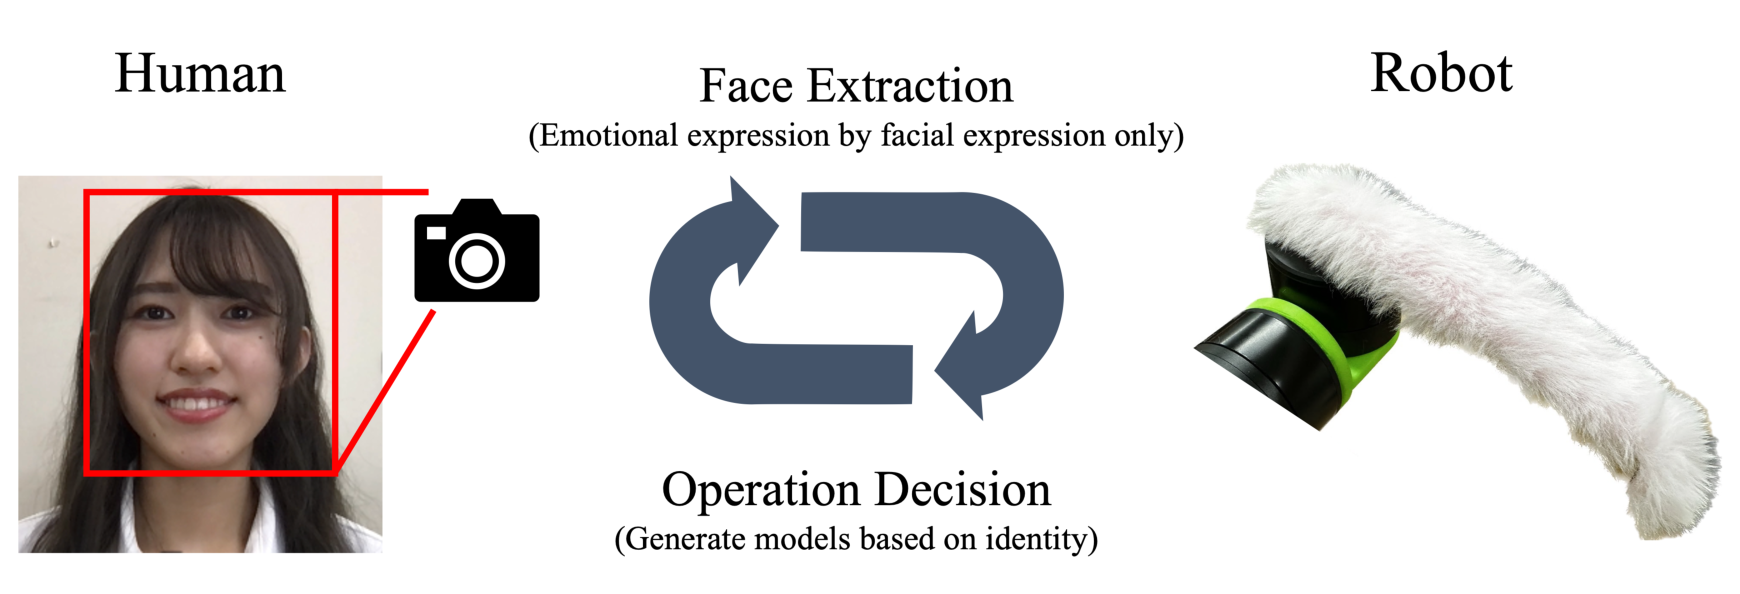
\includegraphics[scale=0.5]{System_new.eps}
\end{center}
\caption{システム概要}
\label{System Overview} %ここでは図のラベルを指定できます。詳しくはこの後記述します。
\end{figure}


%\afterpage{\clearpage}
%%-------------------------------------------------------------------------------------------------------------
%\newpage
%% トレーニング %%

\subsection{計測画像からの表情の認識}
まず,計測画像から表情の認識を行う.システムの構成図を図\ref{System Face}に示す.システムは,カメラ(Logicool C922n)から得られる動画像から,クラウドプラットフォーム(Amazon Web Services:以下AWSを略記)を利用して感情推定を行い,推定結果をリアルタイムでフィードバックする.表情の表現力トレーニングシステムの一例として,入力した動画像と推定結果のフィードバック画面を図\ref{System 3}に示す.


%%--------------------------------------------------画像-------------------------------------------------------
\begin{figure}[h]
\begin{center}
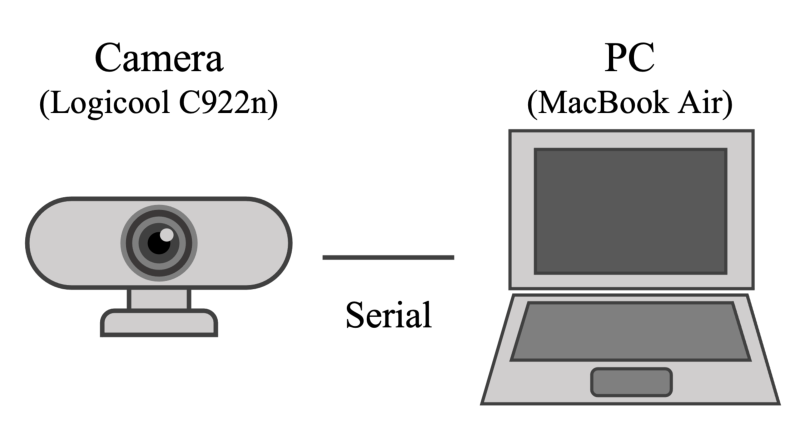
\includegraphics[scale=0.8]{System_Face.eps}
\end{center}
\caption{システム構成図}
\label{System Face} %ここでは図のラベルを指定できます。詳しくはこの後記述します。
\end{figure}

\begin{figure}[h]
\begin{center}
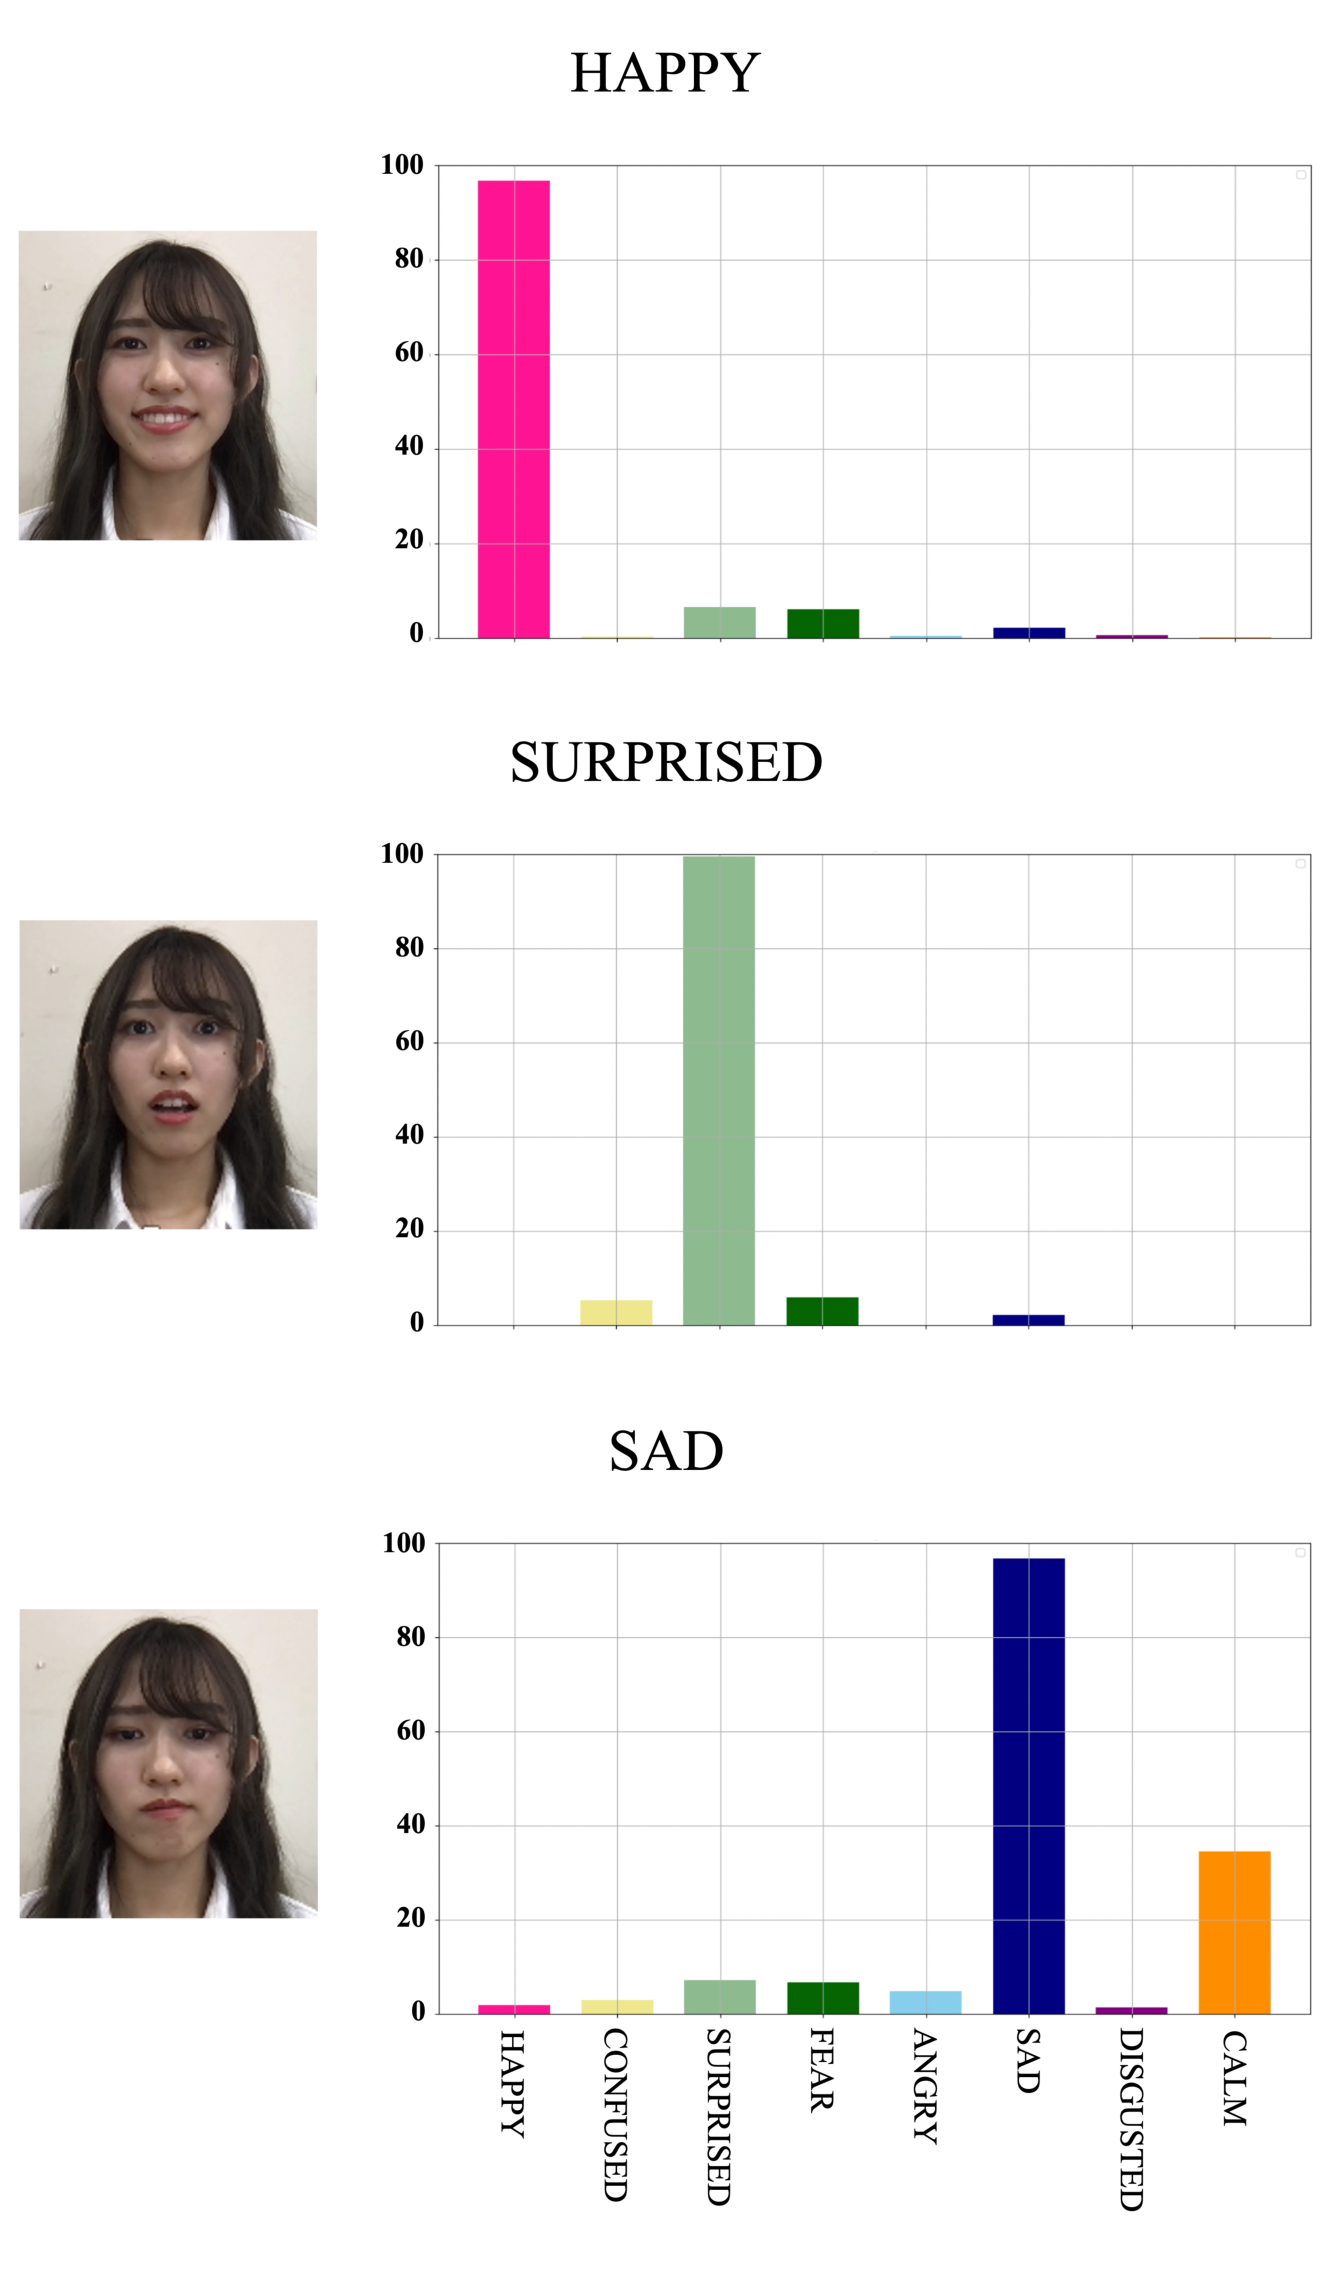
\includegraphics[scale=0.5]{System_3.eps}
\end{center}
\caption{入力動画像とインターフェース画面}
\label{System 3} %ここでは図のラベルを指定できます。詳しくはこの後記述します。
\end{figure}

\afterpage{\clearpage}
%%-------------------------------------------------------------------------------------------------------------
\newpage
\subsection{感情表現に基づくロボット制御}
感情表現に基づき人とインタラクションするロボットを制御した.作成したロボットを図\ref{Robot}に示す.

システムの構成図を図\ref{System Robot}に示す.システムは,カメラ(Logicool C922n)から得られる動画像から,クラウドプラットフォーム(AWS)を利用して感情推定を行い,その推定結果に基づいて,ワンボードマイコン(Rasberry Pi 3 Model B)で,サーボモータ(KeiganMotor KM-1S)を制御する.サーボモータをBluetooth接続で制御する際の,BLEライブラリの対応OSがLinuxであるため,ワンボードマイコンを用いた.

図\ref{Robot}で示したロボットはMotor 1は左右運動,Motor 2は上下運動を制御する.図\ref{Robot}で示したロボットの動作一覧を表\ref{Servo Control}に示す.サーボモータの動作一覧は,一般的な共通認識が得られる犬の生態を基に作成した.モータ動作の一例として,入力した動画像とロボットの動作イメージを図\ref{Robot 3}に示す.


\afterpage{\clearpage}

%%--------------------------------------------------画像-------------------------------------------------------
\begin{figure}[h]
\begin{center}
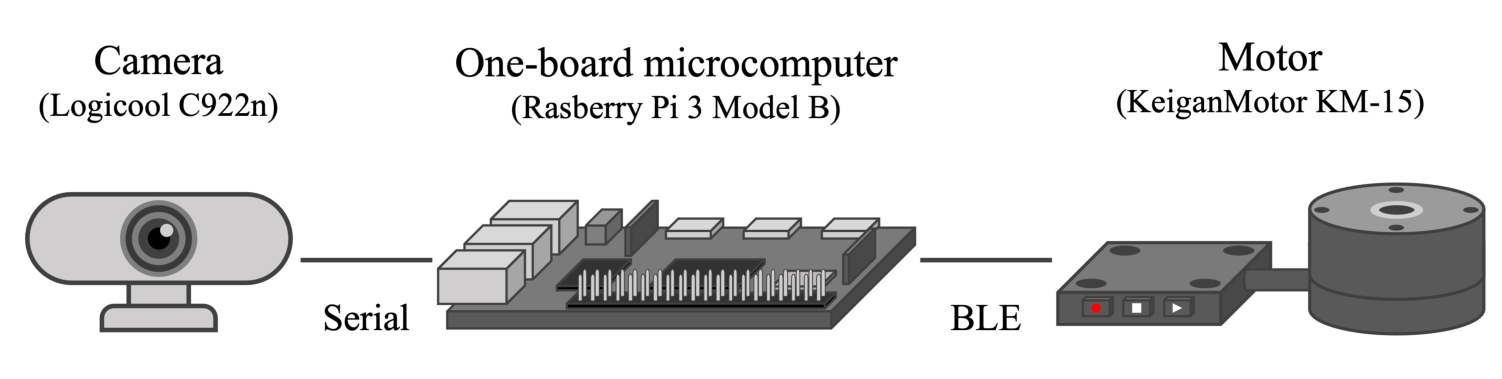
\includegraphics[scale=0.6]{System_Robot.eps}
\end{center}
\caption{システム構成図}
\label{System Robot} %ここでは図のラベルを指定できます。詳しくはこの後記述します。
\end{figure}

\begin{figure}[h]
\begin{center}
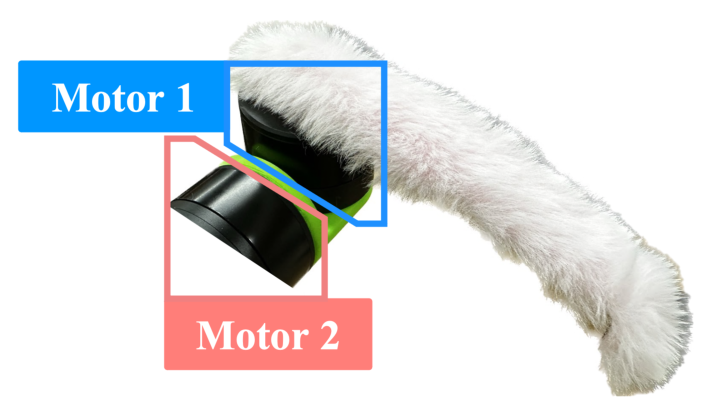
\includegraphics[scale=1.0]{System_robot_motor.eps}
\end{center}
\caption{ロボット}
\label{Robot} %ここでは図のラベルを指定できます。詳しくはこの後記述します。
\end{figure}

\begin{table}[h]
\centering
\caption{動作一覧}
\begin{tabular}{|c||c|c|c|}
    \hline
		感情 & 表現動作 & 左右運動 & 上下運動 \\
	\hline
	\hline
		HAPPY & 尻尾を上げて,振る. & ○ & 上\\
	\hline
		CONFUSED \& ANGRY \& DISGUSTED & 尻尾を下げて,振らない. & × & 下 \\
	\hline
		SURPRISED \& FEAR & 尻尾を上げて,振らない. & × & 上 \\
	\hline
		SAD & 尻尾を下げて,振る. &  ○ & 下 \\
	\hline
        CALM & 尻尾を上げて,振らない & × & 中 \\
	\hline
\end{tabular}
\label{Servo Control}
\end{table}

\begin{figure}[h]
\begin{center}
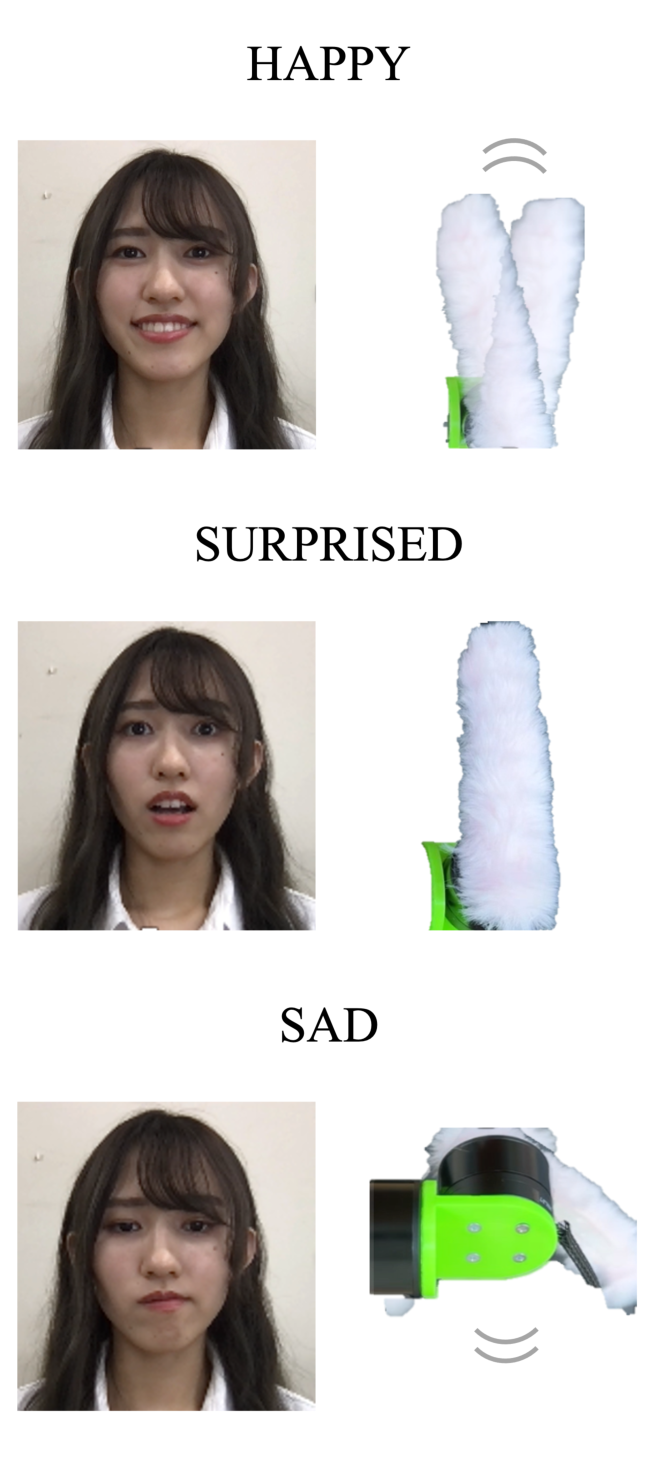
\includegraphics[scale=0.6]{System_robot_new.eps}
\end{center}
\caption{感情に基づいたモータの動作例}
\label{Robot 3} %ここでは図のラベルを指定できます。詳しくはこの後記述します。
\end{figure}

%%-------------------------------------------------------------------------------------------------------------
%%%%%%%%%%%%%

\afterpage{\clearpage}






%%%%%
%%%%%
%********** 3章 *******************************************************************************
%%%%%
%%%%%
\newpage
\section{{検証実験}}

\subsection{感情推定の妥当性と練習の効果}
はじめに,感情表現をインタラクションに使用可能であるかについて,表情認識の精度検証や,表情表出の訓練効果の検証などの基礎的な実験を行った.
実験の条件設定と検証結果について述べる.

\subsubsection{条件}
被験者は20代男性1名とし,指定される感情を5秒間,表情のみで表現する.
指定される感情は,表\ref{Emotion List}に示す8種類である.
実験では,これら8つの各感情をランダムに指定することを1セットとし,3セット実施した.また,表情表出のトレーニング効果も検証するために,表\ref{Experiment environment},図\ref{Jikken1 target}に示す環境で段階的に実験を実施した.実験の際の被験者へのフィードバックは,表\ref{Environment List}に示す4種類とした.フィードバック条件の見本で使用した画像を図\ref{Jikken1 mihon}に示す.

実験は3段階で実施し,表\ref{Environment List}に示すフィードバックを組み合わせて,(a)なし,(b)鏡\&見本,(c)鏡\&見本\&推定結果,の条件を設定し,順番に実施した.
実験風景は,図\ref{Jikken1 3}に示す.

%図と表----------------------------------------
\begin{table}[h]
\centering
\caption{指定される感情一覧}
\begin{tabular}{|c||c|}
    \hline
		 & 感情 \\
	\hline
	\hline
		(1) & HAPPY \\
	\hline
		(2) & CONFUSED \\
	\hline
		(3) & SURPRISED \\
	\hline
		(4) & FEAR \\
	\hline
        (5) & ANGRY \\
	\hline
        (6) & SAD \\
	\hline
        (7) & DISGUSTED \\
	\hline
        (8) & CALM \\
	\hline
\end{tabular}
\label{Emotion List}
\end{table}

\begin{table}[h]
\centering
\caption{実験段階}
\begin{tabular}{|c|c|c|}
	\hline
		(a) & 通常 & 練習やフィードバックを行わない \\
	\hline
		(b) & 練習 & 鏡や見本を提示し,自身で練習 \\
	\hline
		(c) & 評価 & 推定結果をフィードバックに基づいて練習 \\
	\hline
\end{tabular}
\label{Experiment environment}
\end{table}


\begin{figure}[h]
\begin{center}
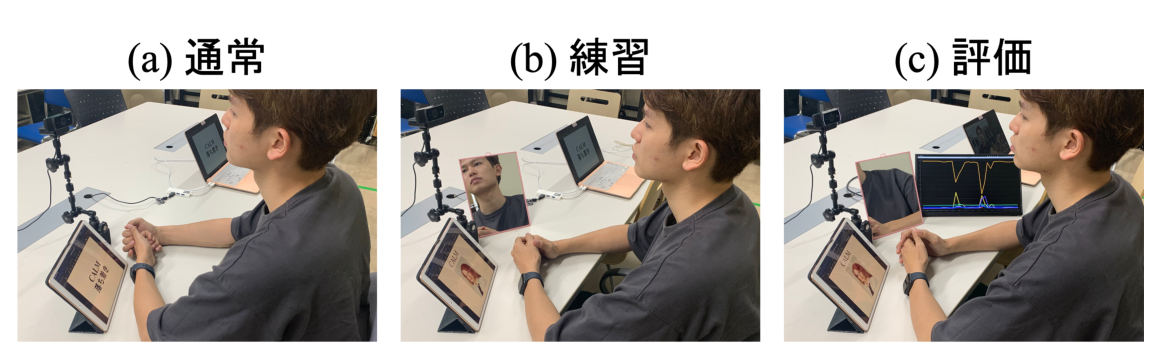
\includegraphics[scale=0.2]{Jikken1_target.eps}
\end{center}
\caption{実験段階イメージ}
\label{Jikken1 target} %ここでは図のラベルを指定できます。詳しくはこの後記述します。
\end{figure}

\begin{table}[h]
\centering
\caption{フィードバック条件}
\begin{tabular}{|c|c|}
    \hline
		フィードバック方法 & 説明 \\
	\hline
	\hline
		推定結果 & リアルタイムで結果をフィードバック \\
	\hline
		鏡 & 被験者が自身の顔を確認 \\
	\hline
		見本 & 8種類の典型的な表情が提示される \\
	\hline
		なし & フィードバックを行わない\\
	\hline
\end{tabular}
\label{Environment List}
\end{table}

\begin{figure}[h]
\begin{center}
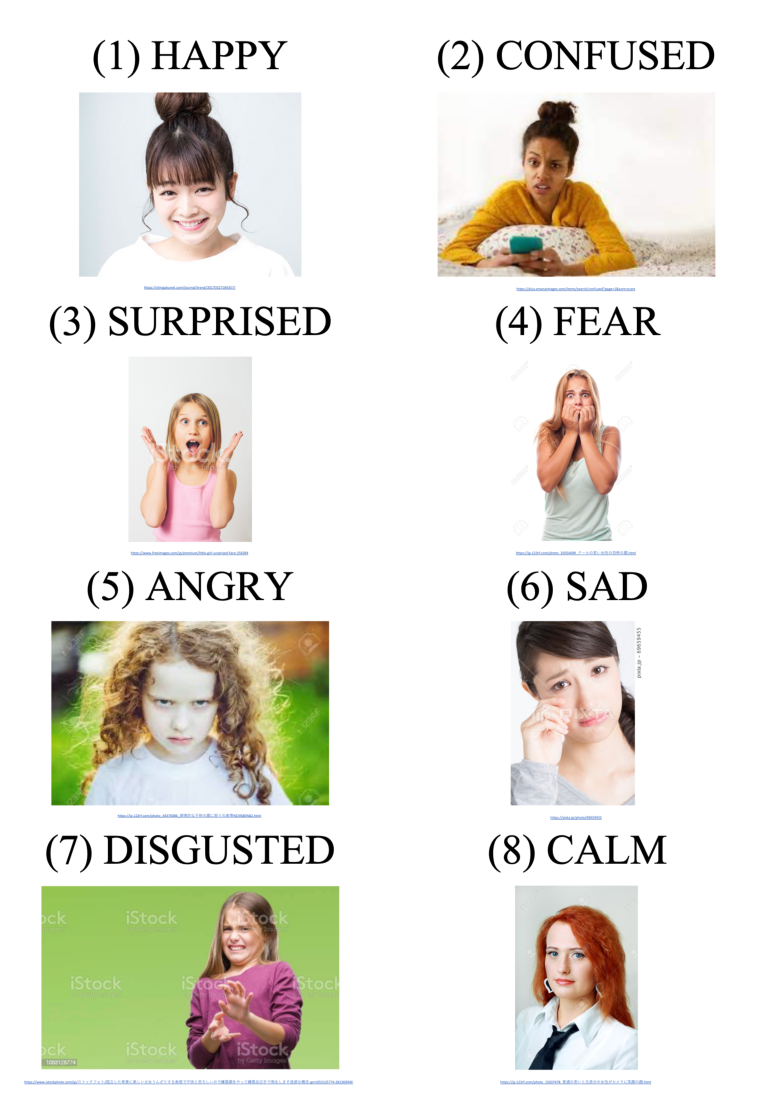
\includegraphics[scale=0.8]{Jikken1_mihon.eps}
\end{center}
\caption{フィードバックに用いた見本の一覧}
\label{Jikken1 mihon} %ここでは図のラベルを指定できます。詳しくはこの後記述します。
\end{figure}

\begin{figure}[h]
\begin{center}
\includegraphics[scale=0.6]{Jikken1_3.eps}
\end{center}
\caption{実験風景}
\label{Jikken1 3} %ここでは図のラベルを指定できます。詳しくはこの後記述します。
\end{figure}

%---------------------------------------------

\afterpage{\clearpage}
\newpage

\subsubsection{検証結果}
被験者に指定した感情と,推定結果が一致した割合を正解率とする.各条件下での感情毎の正解率を図\ref{Jikken1}に示す.各条件下での正解率,適合率,再現率,F値を表\ref{Jikken1_accuracy}に示す.フィードバックなしの環境での,正解率は33.3$%$であった.鏡\&見本の環境での,正解率は58.3$%$であり,フィードバックなしの環境と比較すると,正解率は25.0$%$上昇した.また,鏡\&見本\&推定結果の環境での,正解率は91.7$%$であり,フィードバックなしの環境と比較すると,正解率は58.3$%$と大幅に上昇した.これらの結果から,練習を行うだけでなく,評価を加えることにより高精度な感情推定が可能となることが示された.

%図と表%%%%%%%%%%%%%%%%%%%%%%%%%%%%%%%%%%%%

\begin{figure}[h]
\begin{center}
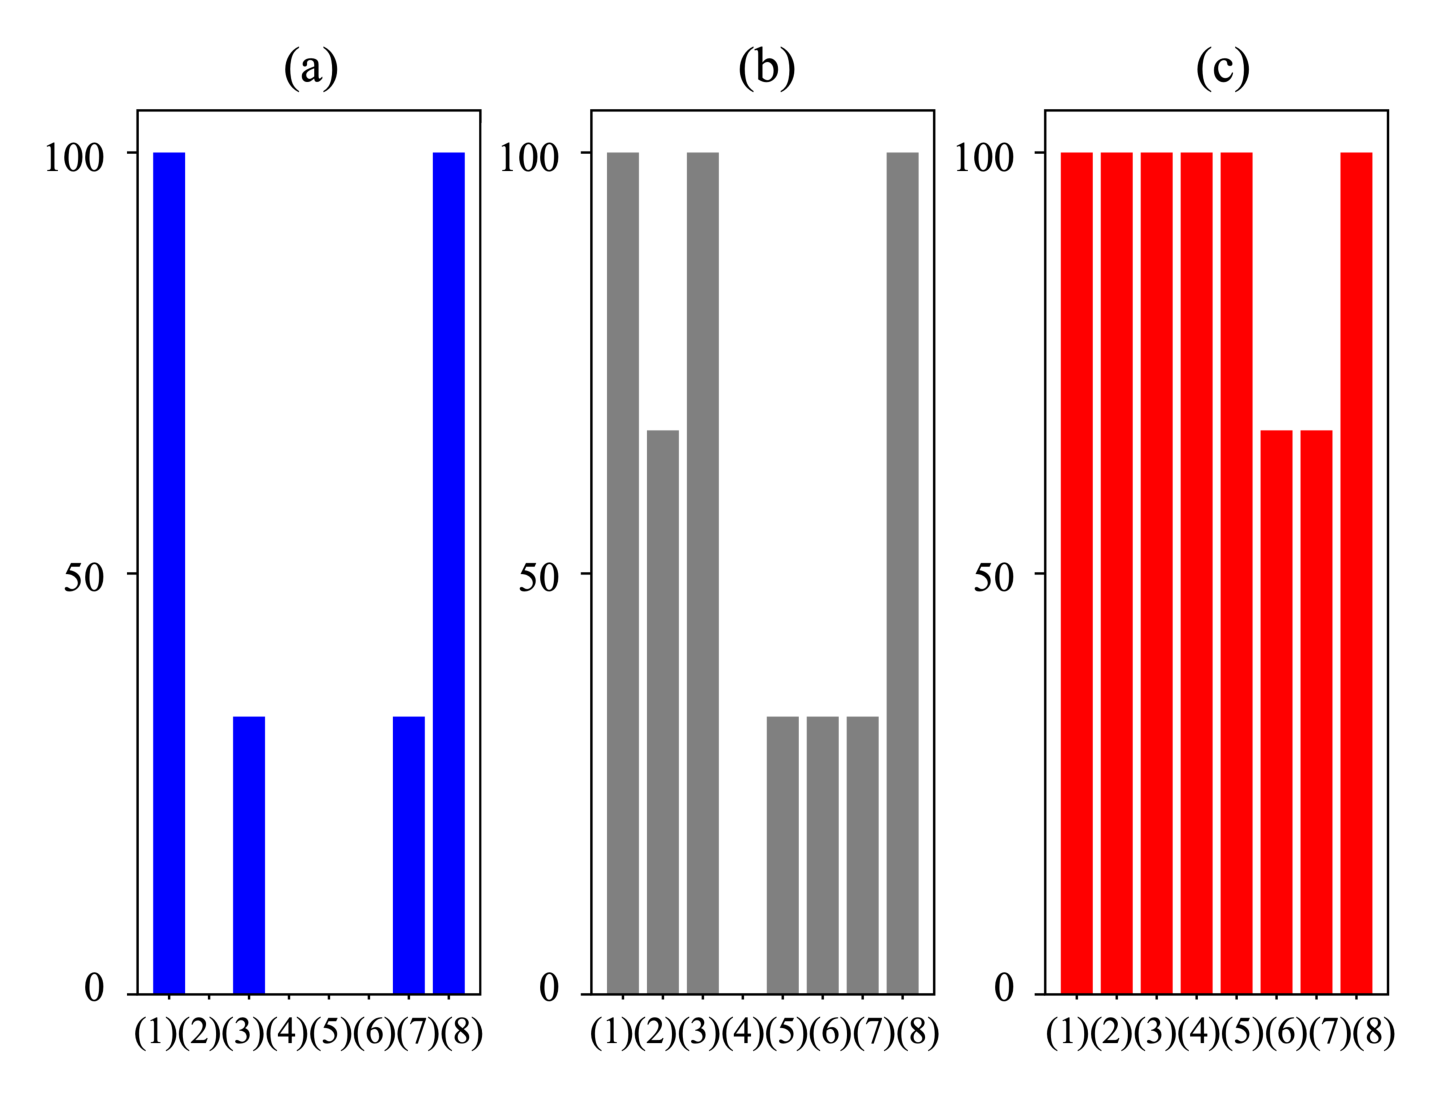
\includegraphics[scale=0.6]{Jikken1.eps}
\end{center}
\caption{各感情下での感情認識結果}
\label{Jikken1} %ここでは図のラベルを指定できます。詳しくはこの後記述します。
\end{figure}


\begin{table}[h]
\centering
\caption{各条件下での認識精度}
\begin{tabular}{|c||c|c|c|}
	\hline
         & (a)なし & (b)鏡\&見本 & (c)鏡\&見本\&推定結果\\
    \hline
    \hline
		Accuracy & 33.3$%$ & 58.3$%$ & 91.7$%$\\
	\hline
		Precision & 0.39 & 0.54  & 0.95\\
	\hline
		Recall & 0.33 & 0.58 & 0.92 \\
	\hline
		F-measure & 0.30 & 0.52 & 0.92\\
	\hline
\end{tabular}
\label{Jikken1_accuracy}
\end{table}

%---------------------------------------------

\afterpage{\clearpage}
\newpage

\subsection{AIと人間との感情推定の相関}
次に,人とAWSによる感情推定の整合性について基礎的な検証を行った.
検証の条件設定と検証結果について述べる.

\subsubsection{条件}
3.1の検証実験で撮影した動画像を複数の第三者に視聴させ,感情を推定する.第三者は20代男女3名とし,動画像は計72種類視聴させた.動画像は,3.1の検証実験の被験者のみ写っており,動画像のイメージを図\ref{Jikken2 movie}に示す.72種類の動画像は,3段階の実験でそれぞれ撮影した,8種類の感情を3回ずつ表現したものである.

%図と表%%%%%%%%%%%%%%%%%%%%%%%%%%%%%%%%%%%%
\begin{figure}[h]
\begin{center}
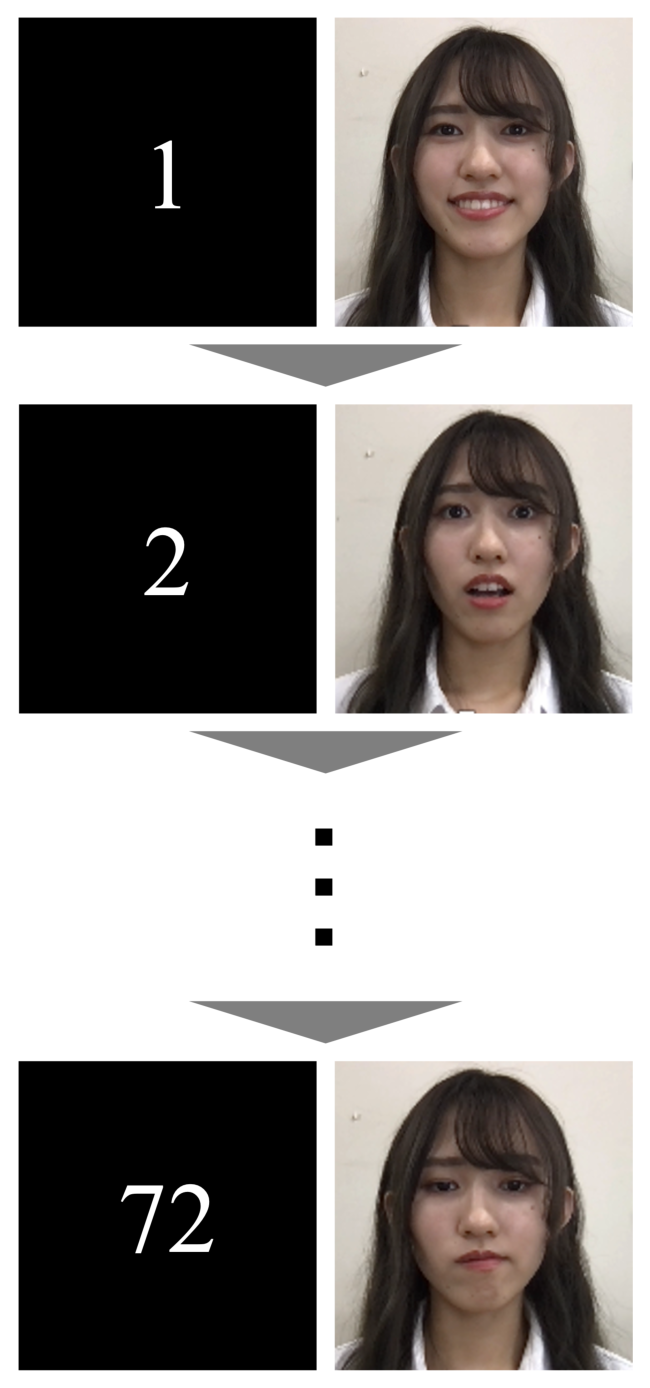
\includegraphics[scale=0.9]{Jikken2_movie.eps}
\end{center}
\caption{動画像イメージ}
\label{Jikken2 movie} %ここでは図のラベルを指定できます。詳しくはこの後記述します。
\end{figure}
%%%%%%%%%%%%%%%%%%%%%%%%%%%%%%%%%%%%%%%%%%

\subsubsection{検証結果}
AWSの感情推定の結果と,第三者の感情推定の結果が一致した割合を正解率とする.各条件下での正解率を図\ref{Jikken2}に示す.縦軸がAWS,横軸が第三者による感情推定の結果である.各条件下での正解率,適合率,再現率,F値を表\ref{Jikken2_accuracy}に示す.

フィードバックなしの環境での,正解率は26.4$%$であった.鏡\&見本の環境での,正解率は52.8$%$であり,フィードバックなしの環境と比較すると,正解率は26.4$%$上昇した.また,鏡\&見本\&推定結果の環境での,正解率は54.2$%$であり,フィードバックなしの環境と比較すると,正解率は27.8$%$と大幅に上昇した.これらの結果から,人とAWSによる感情推定の結果は必ずしも一致しなかったが,HAPPYやSURPRISED,SAD,DISGUSTEDには練習による推定精度の向上と,人の推定結果との整合性が確認された.これらは,感情表現に基づくインタラクションの候補とできることが示唆された.

%図と表%%%%%%%%%%%%%%%%%%%%%%%%%%%%%%%%%%%%
%1
\begin{figure}[h]
\begin{center}
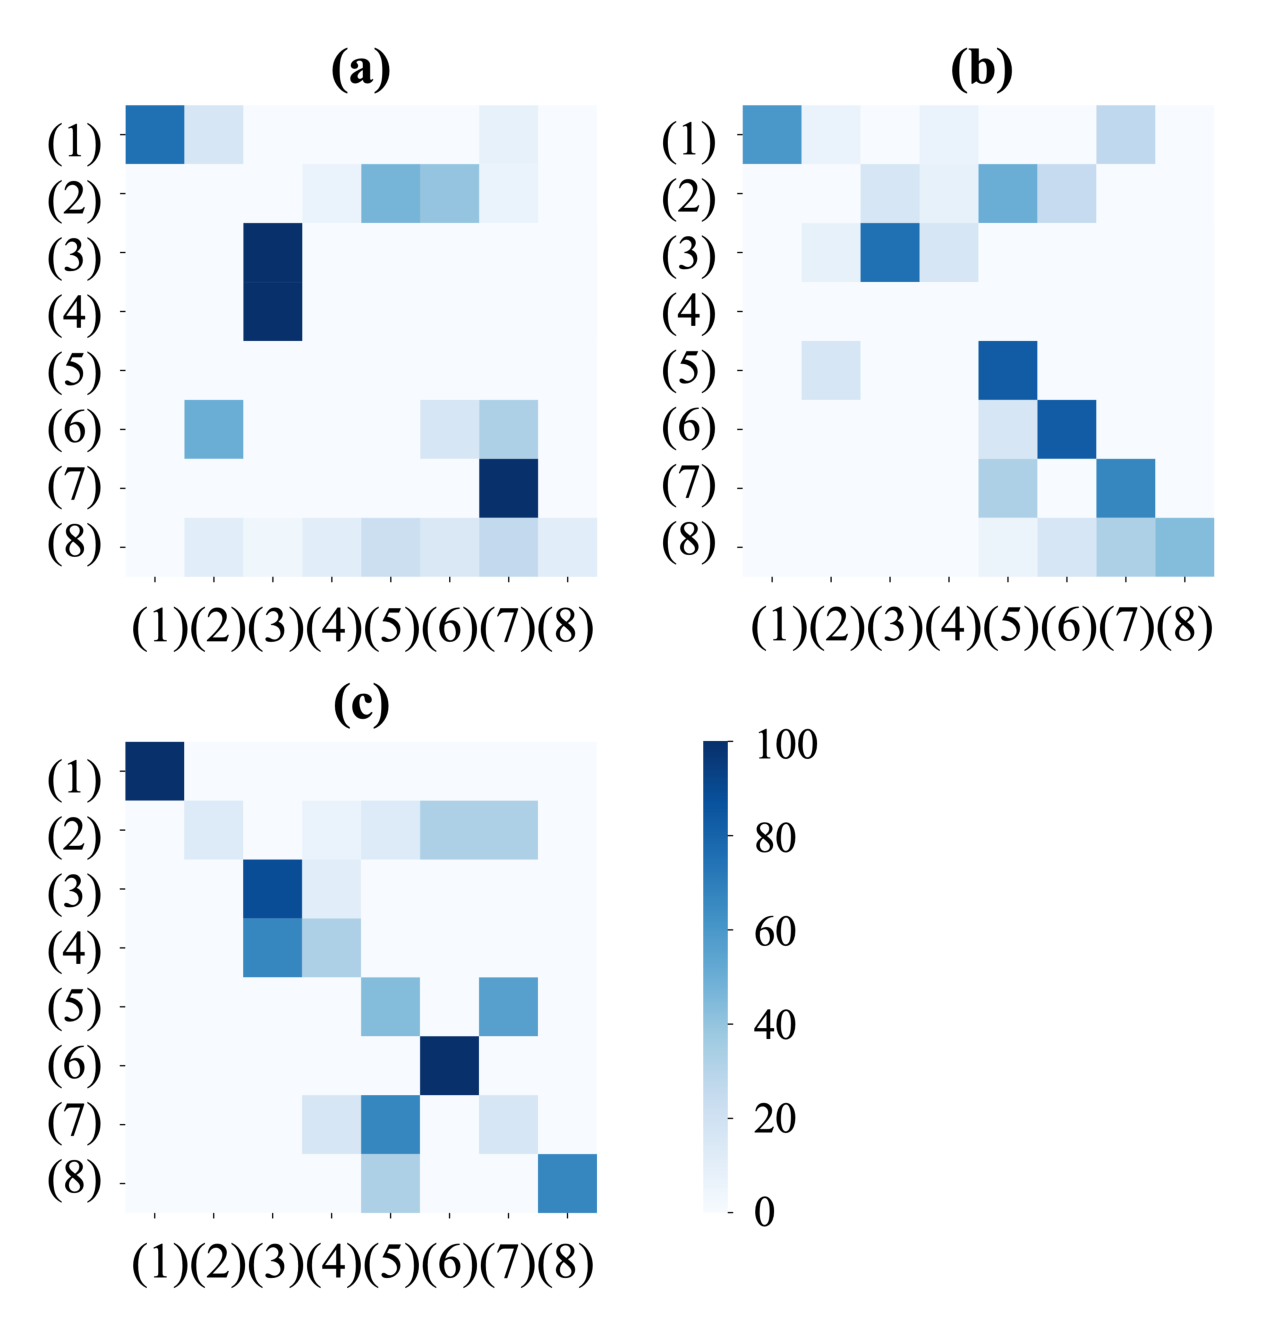
\includegraphics[scale=0.7]{Jikken2.eps}
\end{center}
\caption{第三者とAWSによる感情推定の整合性の検証結果}
\label{Jikken2} %ここでは図のラベルを指定できます。詳しくはこの後記述します。
\end{figure}

\begin{table}[h]
\centering
\caption{各条件下での認識精度}
\begin{tabular}{|c||c|c|c|}
	\hline
         & (a)なし & (b)鏡\&見本 & (c)鏡\&見本\&推定結果\\
    \hline
    \hline
		Accuracy & 26.4$%$ & 52.8$%$ & 54.2$%$\\
	\hline
		Precision & 0.33 & 0.48 & 0.63\\
	\hline
		Recall & 0.38 & 0.52 & 0.58 \\
	\hline
		F-measure & 0.25 & 0.44 & 0.54\\
	\hline
\end{tabular}
\label{Jikken2_accuracy}
\end{table}

%---------------------------------------------

\afterpage{\clearpage}
\newpage

\subsection{感情に基づくロボット制御}
最後に,感情に基づいて行動するロボットを用いたトレーニングを実施し,表現力向上の効果と,心理的な効果について検証を行った.検証の条件設定と検証結果について述べる.

\subsubsection{条件}
被験者は20代男女10名とした.被験者は,各々表情表出トレーニングを5分間行う.トレーニングの前後では,3.1と同様に,指定される感情を5秒間,表情のみで表現する.指定される感情は,表\ref{Emotion List 2}に示す5種類である.AWSでは,8種類の感情を推定することができるが,3.1,3.2の検証から,第三者とAWSによる感情推定では,類似した特徴を持つ表情は,どちらの感情推定でも相互に誤認識をを生じることが多い.そこで,類似した特徴を持つ表情を統合し,5種類とした.実験では,これら5つの各感情をランダムに指定することを1セットとして,トレーニングの前後で,2セットずつ行った.

被験者がトレーニングを行う際のフィードバックの方法は,表\ref{Environment List 2}に示す2種類とした.実験風景を図\ref{Jikken3 2}に示す.ロボットでのトレーニングでは,ロボットの動作とイラストによるフィードバックを同時に行った.その際のフィードバック内容を図\ref{Jikken3 Image}に示す.フィードバック条件が鏡でのトレーニング終了後,48時間以上経過後に,フィードバック条件がロボットでのトレーニングを実施した.

また,被験者に実験の前後にアンケート調査を実施した.アンケート調査では,トレーニング前後での心理状態の調査やトレーニングの満足度調査,表現力向上効果の実感の調査に加え,提案システムに関する調査を行った.アンケート調査の内容は,表\ref{Question List}に示す.1〜20の質問項目は,フィードバック条件が鏡,ロボットの両者の実験において実施した.21〜26の質問項目は,フィードバック条件がロボットの実験において実施した.心理状態に関する調査の質問項目は,1〜5は対人緊張,6〜10は親和感情に関する質問項目を用いた\cite{hayashi}.アンケート調査は,「非常にそう思う」,「ややそう思う」,「どちらとも言えない」,「そう思わない」,「全くそう思わない」の5段階で回答させた.

%%%%%%%%%%%%%%%%%%%%%%%%%%%%%%%%%
\begin{table}[h]
\centering
\caption{指定される感情一覧}
\begin{tabular}{|c||c|}
    \hline
		 & 感情 \\
	\hline
	\hline
		$\rm\,I\,$ & HAPPY \\
	\hline
		$\rm\,II\,$ & ANGRY\&CONFUSED\&DISGUSTED\\
	\hline
		$\rm\,III\,$ & SURPRISED\&FEAR \\
	\hline
		$\rm\,IV\,$ & SAD \\
	\hline
        $\rm\,V\,$  & CALM \\
	\hline
\end{tabular}
\label{Emotion List 2}
\end{table}

\begin{table}[h]
\centering
\caption{フィードバック条件}
\begin{tabular}{|c|c|c|}
    \hline
		&フィードバック方法 & 説明 \\
	\hline
	\hline
		(A) & 鏡 & 被験者が自身の顔を確認 \\
	\hline
		(B) & ロボット & ロボットとイラストで結果を同時にフィードバック \\
	\hline
\end{tabular}
\label{Environment List 2}
\end{table}

\begin{figure}[h]
\begin{center}
\includegraphics[scale=0.9]{Jikken3_2.eps}
\end{center}
\caption{実験風景}
\label{Jikken3 2} 
\end{figure}

\afterpage{\clearpage}
\newpage

\begin{figure}[h]
\begin{center}
\includegraphics[scale=0.5]{Jikken3_robot_image.eps}
\end{center}
\caption{各感情に基づいてフィードバックする内容}
\label{Jikken3 Image} 
\end{figure}

\begin{table}[h!]
\centering
\caption{アンケート内容}
\begin{tabular}{|c||cc|}
    \hline
        \multirow{10}{*}{心理特性調査} & Q1 & 緊張する\\
        & Q2 & 堅苦しい\\
        & Q3 & 苦手である\\
        & Q4 & 気軽である\\
        & Q5 & 疲れる\\
        & Q6 & 孤独を和らげる\\
        & Q7 & 楽しい\\
        & Q8 & 気軽に心を開ける\\
        & Q9 & 集中できる\\
        & Q10 & 感情を表現しやすい\\
	\hline
        \multirow{5}{*}{満足度調査} & Q11 & トレーニングを楽しく行えたか\\
        & Q12 & 表現力が向上したと感じるか\\
        & Q13 & 継続しやすいと思うか\\
        & Q14 & トレーニングとして満足できたか\\
        & Q15 & また使いたいと思うか\\
    \hline 
        \multirow{5}{*}{トレーニング効果調査} & Q16 & HAPPY \\
		& Q17 & ANGRY\&CONFUSED\&DISGUSTED\\
		& Q18 & SURPRISED\&FEAR \\
		& Q19 & SAD \\
        & Q20 & CALM \\
    
    \hline
        \multirow{6}{*}{システム調査} & Q21 & ロボットに意思を伝えることはできたか\\
        & Q22 & 思い通りに制御できたか\\
        & Q23 & 触れ合いは楽しかったか\\
        & Q24 & 動作が適切であったか\\
        & Q25 & その他フィードバックは適切であったか\\
        & Q26 & フィードバックの注目度\\
    \hline
        
\end{tabular}
\label{Question List}
\end{table}

%%%%%%%%%%%%%%%%%%%%%%%%%%%%%%%%%
\afterpage{\clearpage}
%%-------------------------------------------------------------------------------------------------------------
\newpage

\subsubsection{検証結果}
%図の追加
被験者に指定した感情と,推定結果が一致した割合を正解率とする.トレーニング前をBefore,トレーニング後をAfterとする.各条件下でのトレーニング前後での感情毎の正解率を図\ref{Jikken3}に示す.各条件下でのトレーニング前後の正解率,適合率,再現率,F値を表\ref{Jikken3_accuracy}に示す.鏡でのトレーニング前の,正解率は62.6$%$であった.鏡でのトレーニング後の,正解率は64.0$%$であり,トレーニング前と比較すると,正解率は1.4$%$上昇した.ロボットでのトレーニング前の,正解率は68.0$%$であった.ロボットでのトレーニング後の,正解率は77.0$%$であり,トレーニング前と比較すると,正解率は9.0$%$上昇した.鏡でのトレーニング前後では,正解率の上昇は,$\rm\,II\,$,$\rm\,III\,$の感情で見られた.しかし,フィードバックの受け止め方が個人の主観に依存するため,誤った表情をトレーニングしてしまい,正解率が低下した感情もある結果となった.一方,ロボットでのトレーニング前後では,正解率の上昇が$\rm\,II\,$,$\rm\,III\,$,$\rm\,IV\,$の感情で見られ,表出が困難と思われる$\rm\,II\,$,$\rm\,IV\,$においてともに20.0$%$以上の大幅な上昇が見られた.しかし,システムからの評価を客観的にフィードバックしたものの,鏡のトレーニングと同様に,誤った表情をトレーニングしてしまい,正解率が低下した感情もある結果となった.

また,各条件下でのトレーニング前後でのアンケート調査の結果を図\ref{Jikken3_Q1}〜図\ref{Jikken3_Q3}に示す.心理特性において,トレーニング前後での平均値を比較するとBeforeよりAfterの方が,「Q1:緊張する」,「Q2:堅苦しい」,「Q3:苦手である」,「Q5:疲れる」などのマイナスな質問項目は低下し,「Q4:気軽である」,「Q6:孤独を和らげる」,「Q7:楽しい」,「Q8:気軽に心を開ける」,「Q9:集中できる」,「Q10:感情を表現しやすい」などのプラスな質問項目は上昇した.トレーニング環境での平均値を比較すると鏡でのトレーニング環境よりロボットでのトレーニング環境の方が,トレーニング前後での平均値の比較と同様に,マイナスな質問項目は低下し,プラスな質問項目は上昇した.

次に,満足度調査において,トレーニング環境を比較すると,鏡でのトレーニング環境よりロボットでのトレーニング環境の方が「Q11:トレーニングを楽しく行なうことができたか」,「Q12:表現力が向上したと感じるか」,「Q13:継続しやすいと思うか」,「Q14:トレーニングとして満足できたか」,「Q15:また使いたいと思うか」で平均値が上昇し,満足度が高まり,100$%$の人が「表現力が高まったと実感する」と回答した.

トレーニング効果調査において,トレーニング環境を比較すると,鏡でのトレーニング環境よりロボットでのトレーニング環境の方が「Q16:HAPPY」,「Q17:ANGRY\&CONFUSED\&DISGUSTED」,「Q18:SURPRISED\&FEAR」,「Q19:SAD」,「Q20:CALM」で平均値が上昇し,各感情において表現力の向上を実感しているという結果が得られた.

最後に,システム調査において,ロボットでのトレーニング環境では,「Q21:ロボットに意思を伝えることができたか」,「Q22:思い通りに制御できたか」,「Q23:触れ合いは楽しかったか」,「Q24:動作が適切であったか」,「Q25:その他フィードバックは適切であったか」では,全体的にシステムに満足できる結果となった.また,「Q26:トレーニング時の注目度」は,ややロボット優勢の結果となり,ロボットでのフィードバックに好意的な意見が多く聞かれた.その一方で,「フィードバックまでの時差」や「フィードバック方法・位置」などのシステムの問題点が挙げられた.

%図と表%%%%%%%%%%%%%%%%%%%%%%%%%%%%%
%どちらか%%%%
\begin{figure}[h]
\begin{center}
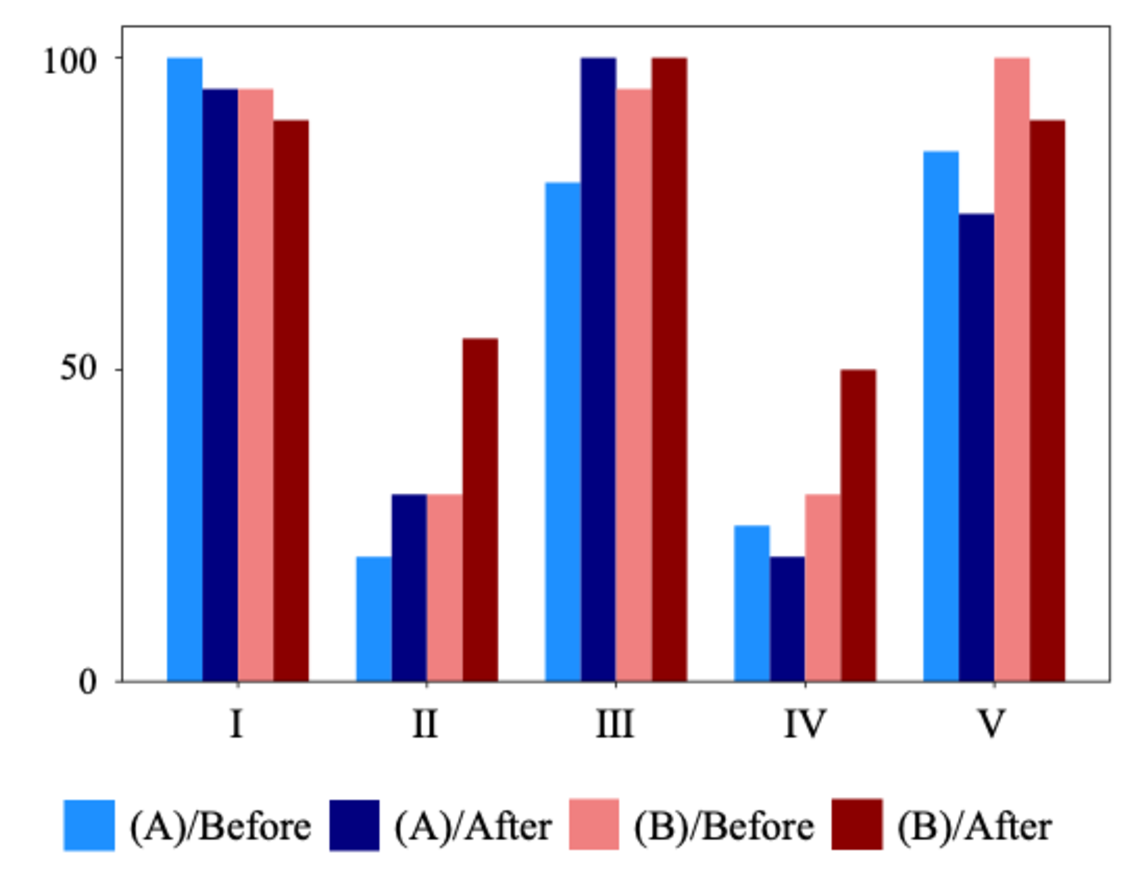
\includegraphics[scale=0.7]{Jikken3.eps}
\end{center}
\caption{トレーニング前後での正解率}
\label{Jikken3} %ここでは図のラベルを指定できます。詳しくはこの後記述します。
\end{figure}

\begin{table}[h]
\centering
\caption{各条件下での認識精度}
\begin{tabular}{|c||cc|cc|}
	\hline
         & \multicolumn{2}{c|}{(A)鏡} & \multicolumn{2}
         {c|}{(B)ロボット}\\
    \hline
         & Before & After & Before & After\\
    \hline
    \hline
		Accuracy & 62.6$%$ & 64.0$%$ & 68.0$%$ & 77.0$%$ \\
	\hline
		Precision & 0.67 & 0.62 & 0.68  & 0.79 \\
	\hline
		Recall & 0.62 & 0.64 &0.68 & 0.77\\
	\hline
		F-measure & 0.60 & 0.61 & 0.66 & 0.76 \\
	\hline
\end{tabular}
\label{Jikken3_accuracy}
\end{table}

%アンケート%%%%
\begin{figure}[h]
\begin{center}
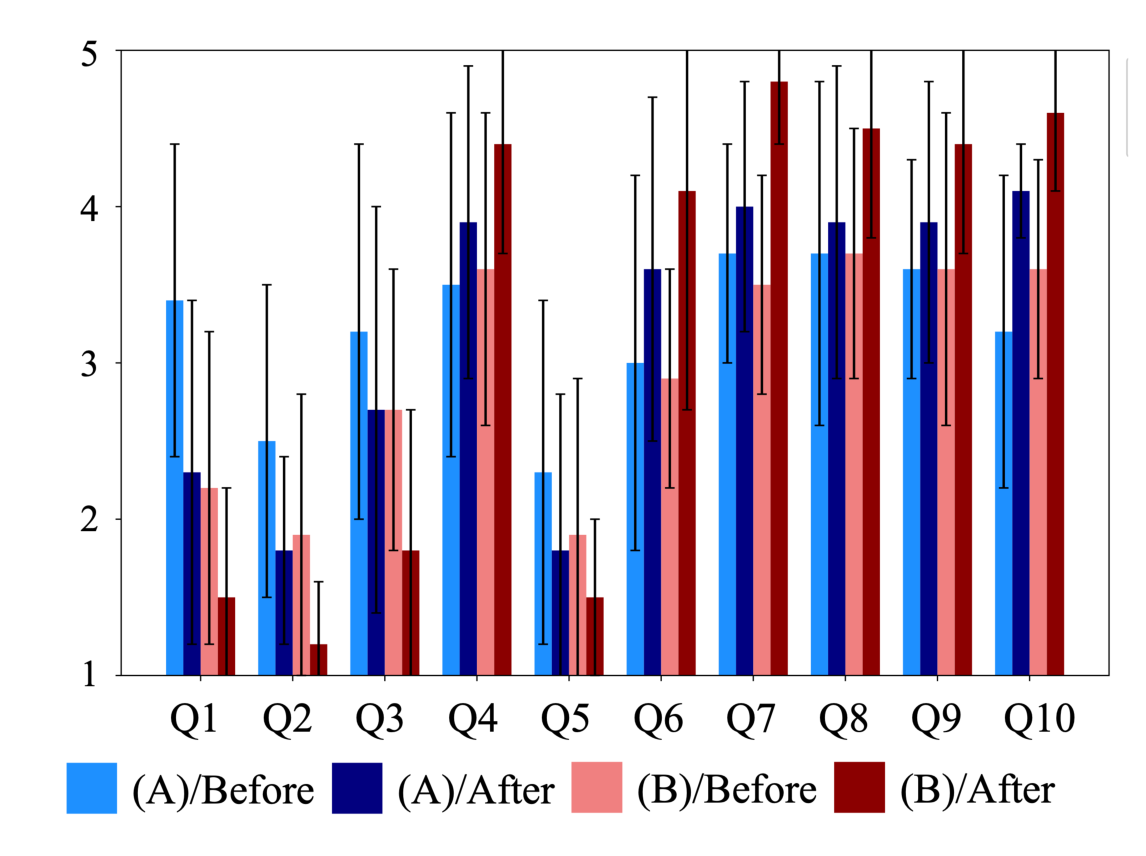
\includegraphics[scale=0.7]{Jikken3_Q1_10.eps}
\end{center}
\caption{心理特性調査}
\label{Jikken3_Q1} %ここでは図のラベルを指定できます。詳しくはこの後記述します。
\end{figure}

\begin{figure}[h]
\begin{center}
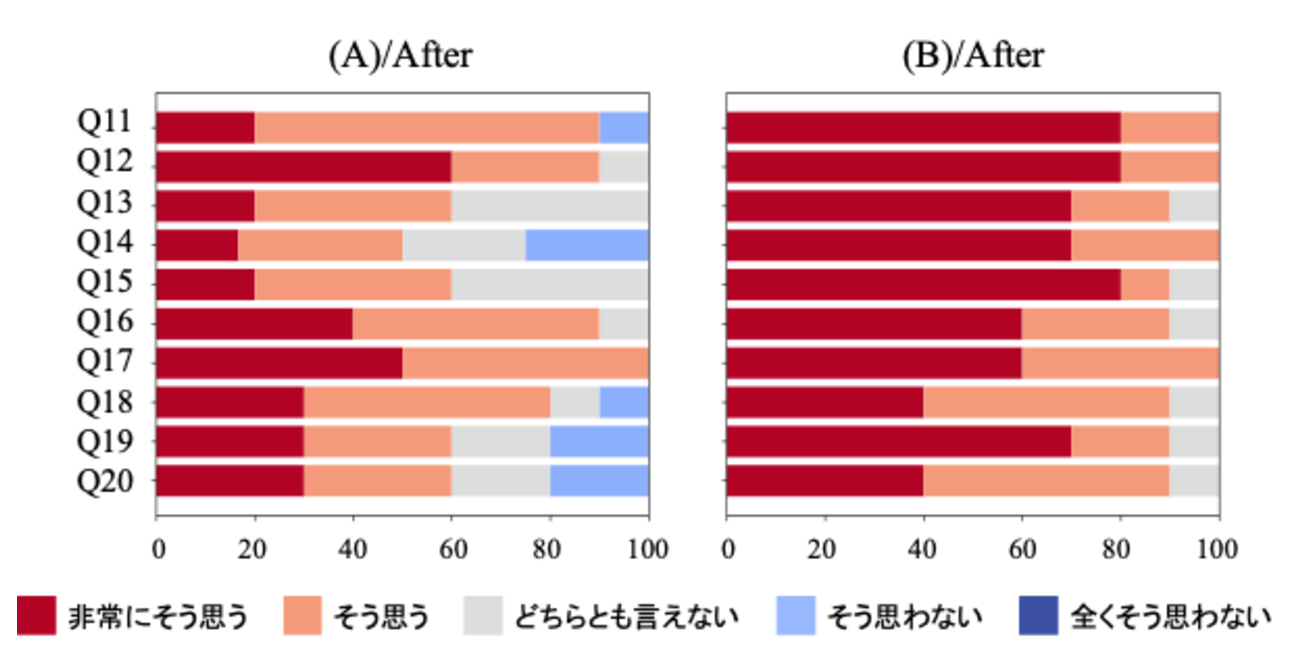
\includegraphics[scale=0.6]{Jikken3_Q11_20.eps}
\end{center}
\caption{満足度・トレーニング効果調査}
\label{Jikken3_Q2} %ここでは図のラベルを指定できます。詳しくはこの後記述します。
\end{figure}

\begin{figure}[h]
\begin{center}
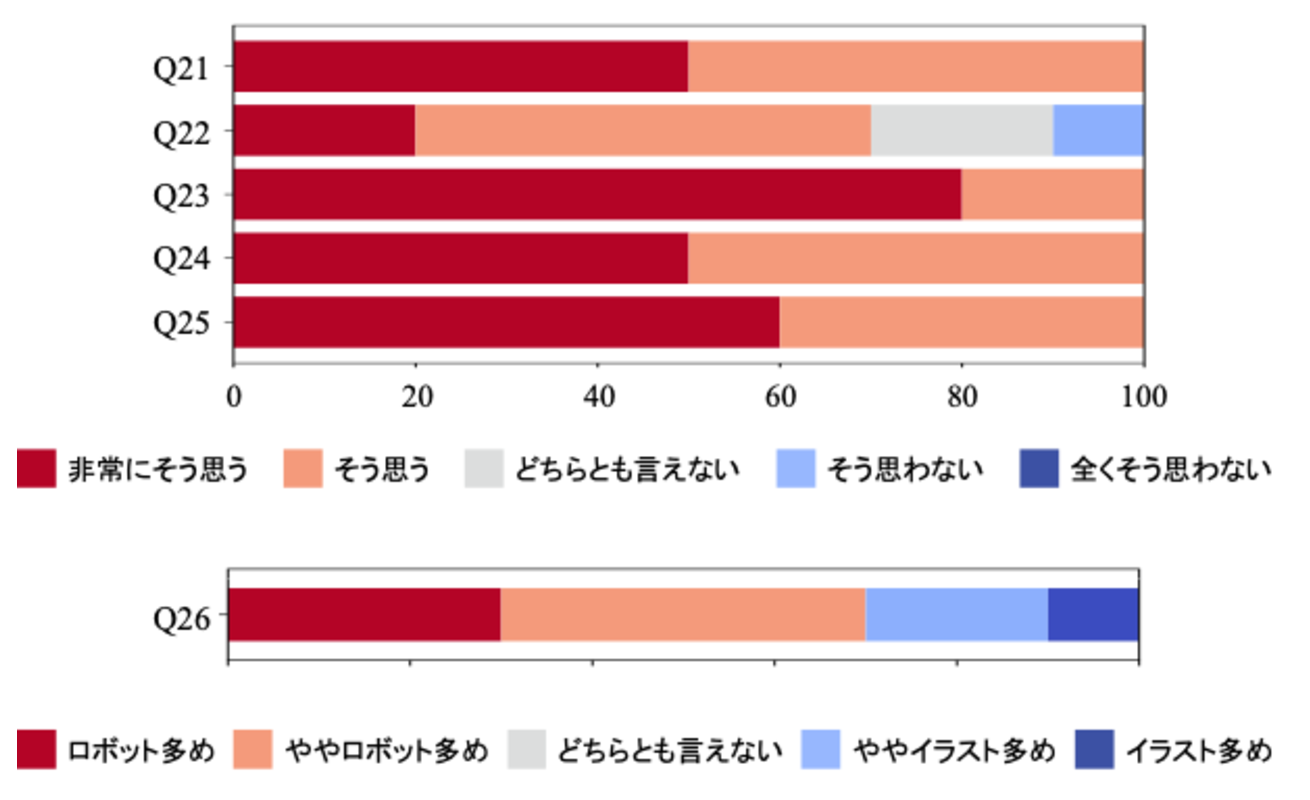
\includegraphics[scale=0.6]{Jikken3_Q21_26.eps}
\end{center}
\caption{システム調査}
\label{Jikken3_Q3} %ここでは図のラベルを指定できます。詳しくはこの後記述します。
\end{figure}
%%%%%%

%%%%%%%%%%%%%%%%%%%%%%%%%%%%%%%%%

\afterpage{\clearpage}
%%%%%
%%%%%
%********** 4章 *******************************************************************************
%%%%%
%%%%%
\clearpage
\section{{まとめ}}
本研究では,感情表現に基づき人とインタラクションするロボットを開発し,表情を表出するトレーニングを日常的に行うことを目指した.表情からの感情推定の精度検証を行い,インタフェース手段として使用可能であることを確認した.また,感情推定結果に基づき,行動するロボットの制作と効果の検証を行った.その結果,ロボットを用いた表情の表出トレーニングの効果を確認し,表出トレーニングにおいてロボットを用いることの有意性を確認した.今後は,ロボットのフィードバック方法の改良を目標とする.

\afterpage{\clearpage}
% 謝辞---------------------------------------------------------------------------------------------------
\newpage
\section*{{謝辞}}
本研究の実施に際して,常日頃より様々なご指導を頂きました福田修教授,Yeoh Wen Liangプロジェクト助教,奥村浩教授,山口暢彦准教授,江藤博文助教,羽根由恵技術員に心から感謝いたします.また,多くのご指摘,ご指導を下さいました佐賀大学理工学部知能情報システム工学コースの皆様に感謝の気持ちとお礼を申し上げたく,謝辞にかえさせていただきます.

 
%********** 参考文献 *****************************************
\newpage
\begin{thebibliography}{99}
\large
{
\bibitem{kaiser}
Kaiser,S., Wehrle,T., Facial Expressions as Indicators of Appraisal Processes, 2001.\\

\bibitem{kawabata}
川畑光代, 桑原尚史, 表情解読プロセスの検討$\rm(\,I\,)$ー表情の認知と心的状態の推論との関係性についてー, 関西大学総合情報学部紀要「情報研究」, 2005\\

\bibitem{kino}
木野和代, 日本人の怒りの表出方法とその対人的影響, 2000\\

\bibitem{endo}
遠藤健治, 表情によるコミュニケーション【ススメ!コミュニケーションの新しいカタチ第1回】, 2020,\\
$https://aogakuplus.jp/column/new_communication_style_20201218_01/$\\(参照 2023-01-17)\\

\bibitem{sato}
佐藤弥, 嶺本和沙, 吉川左紀子,Facial Expressions of Basic Emotions in Japanese Laypeople, 2019\\

\bibitem{takami}
高見愛, 伊藤京子, 西田正吾, 表情トレーニングのための笑顔の定量的評価方法の検討, 2007\\

\bibitem{tashiro}
田代琉人, 牧野貴斗, 大場隆史, 濱川礼, 顔特徴点を利用した表情の表現力向上システム
-POSED LOOK-, 2019\\

\bibitem{fujimoto}
藤本貴大, 大曽彰子, 本山貢, 米山龍介, 松田忠之, 自律高齢者を対象とした介護予防運動プログラムの長期トレーニング効果について, 2008\\

\bibitem{hayashi}
林勇吾, Eric, C. , Victor, V. K., 浦尾彰, 小川均, 対話エージェントとのコミュニケーションにおける心理特性 -スキーマと擬人化に関する検討-, 2012\\

\bibitem{harada}
原田達也, 佐藤和正, 森武俊, 触れ合いロボットによる心理効果 -接触インタラクションによる安心感の演出と痛みの緩和-, 1998\\
}
\end{thebibliography}
\end{document}

